\documentclass[12pt]{article}
\usepackage[margin=1in]{geometry} 
\usepackage{graphicx}
\usepackage{amsmath}
\usepackage{tcolorbox}
\usepackage{amssymb}
\usepackage{amsthm}
\usepackage{lastpage}
\usepackage{fancyhdr}
\usepackage{accents}
\usepackage{float}
\usepackage{xcolor}
\usepackage{ifsym}
\graphicspath{ {./images/} }
\restylefloat{table}
\pagestyle{fancy}
\setlength{\headheight}{42pt}
\newenvironment{solution}
{\renewcommand\qedsymbol{$\blacksquare$}
\begin{proof}[Solution]}
 {\end{proof}}
\renewcommand\qedsymbol{$\blacksquare$}
\newcommand{\ubar}[1]{\underaccent{\bar}{#1}}
\newcommand\noverline[1]{\mkern1mu\overline{\mkern-1mu#1\mkern-1mu}\mkern1mu}
\title{Election Finance Insight:\\Deliverable 2}
\author{Eric Lehmann, Kevin Aukee, \& Daniel Giampaolo}
\begin{document}
\maketitle
%HEADER
%\setcounter{page}{PAGENUMBER}
\lhead{Eric Lehmann, Kevin Aukee, \& Daniel Giampaolo}
\rhead{CIS4301 Spring '20 \\ \today \\ Deliverable 2}
\section{Overview}
Our intent is to design and deploy a web application that allows users to gain insight into the finances of the 2020 Presidential Primary. In an election season with so many candidates, having a tool able to assist in analyzing campaign finance trends would be an invaluable asset. Each candidate is required to report information about individual donations to the Federal Election Commission. This report includes detailed information about each individual donor, including their name, the donation amount, city, and state as well as employer and occupation. We are interested in seeing comparisons to individual campaign events as well as coverage of candidates and their competitors in the news media. Lastly, we believe we will be able to gain insight into the donors by comparing their employers and occupations.
\section{User Interface}
    \begin{figure}[H]
        \begin{center}
        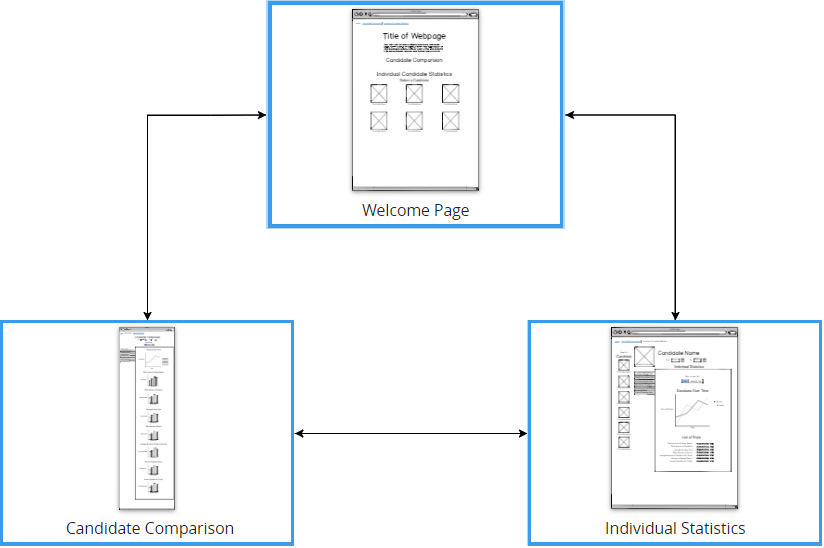
\includegraphics[scale=.60]{EFINode}
        \caption{EFI Diagram}
        \label{fig:EFINode}
        \end{center}
    \end{figure}
    Figure \ref{fig:EFINode} above demonstrates the principal layout of the web site. We intend to offer a landing page, which will present candidates and an option to view either broad candidate comparisons or individual campaign statistics. Links will be available to move back and forth to any page from any page.
    \subsection{Welcome}
    \begin{figure}[H]
        \begin{center}
        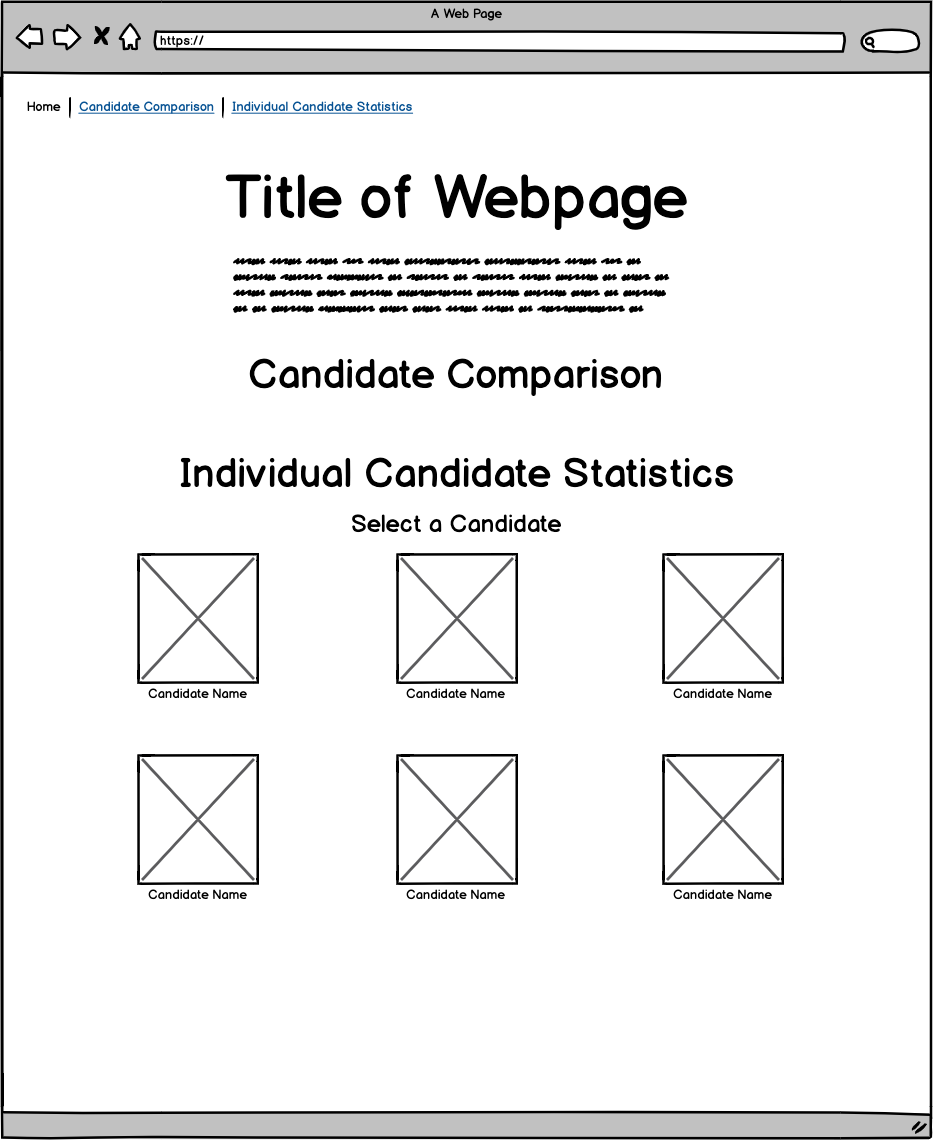
\includegraphics[scale=.30]{welcome}
        \caption{Welcome Page}
        \label{fig:1}
        \end{center}
    \end{figure}
    Our website will start with the users landing on a welcome/home page (Figure \ref{fig:1}). This page has a title and description of the website and a navigation bar at the top to get to the other webpages. Below the title and description will be additional links that will take you to the same webpages as in the navbar. If the user selects the ``Individual Candidate Statistics’’ button on the navbar, the user will be taken to the individual statistics page and the candidate with the largest amount of money raised during the 2020 Presidential Primary will be the default candidate. Otherwise, the user can select a photo of an individual candidate to be directed to the individual candidate page with that specific individual candidate data pulled up right away.
    \subsection{Candidate Comparison}
    \begin{figure}[H]
        \begin{center}
        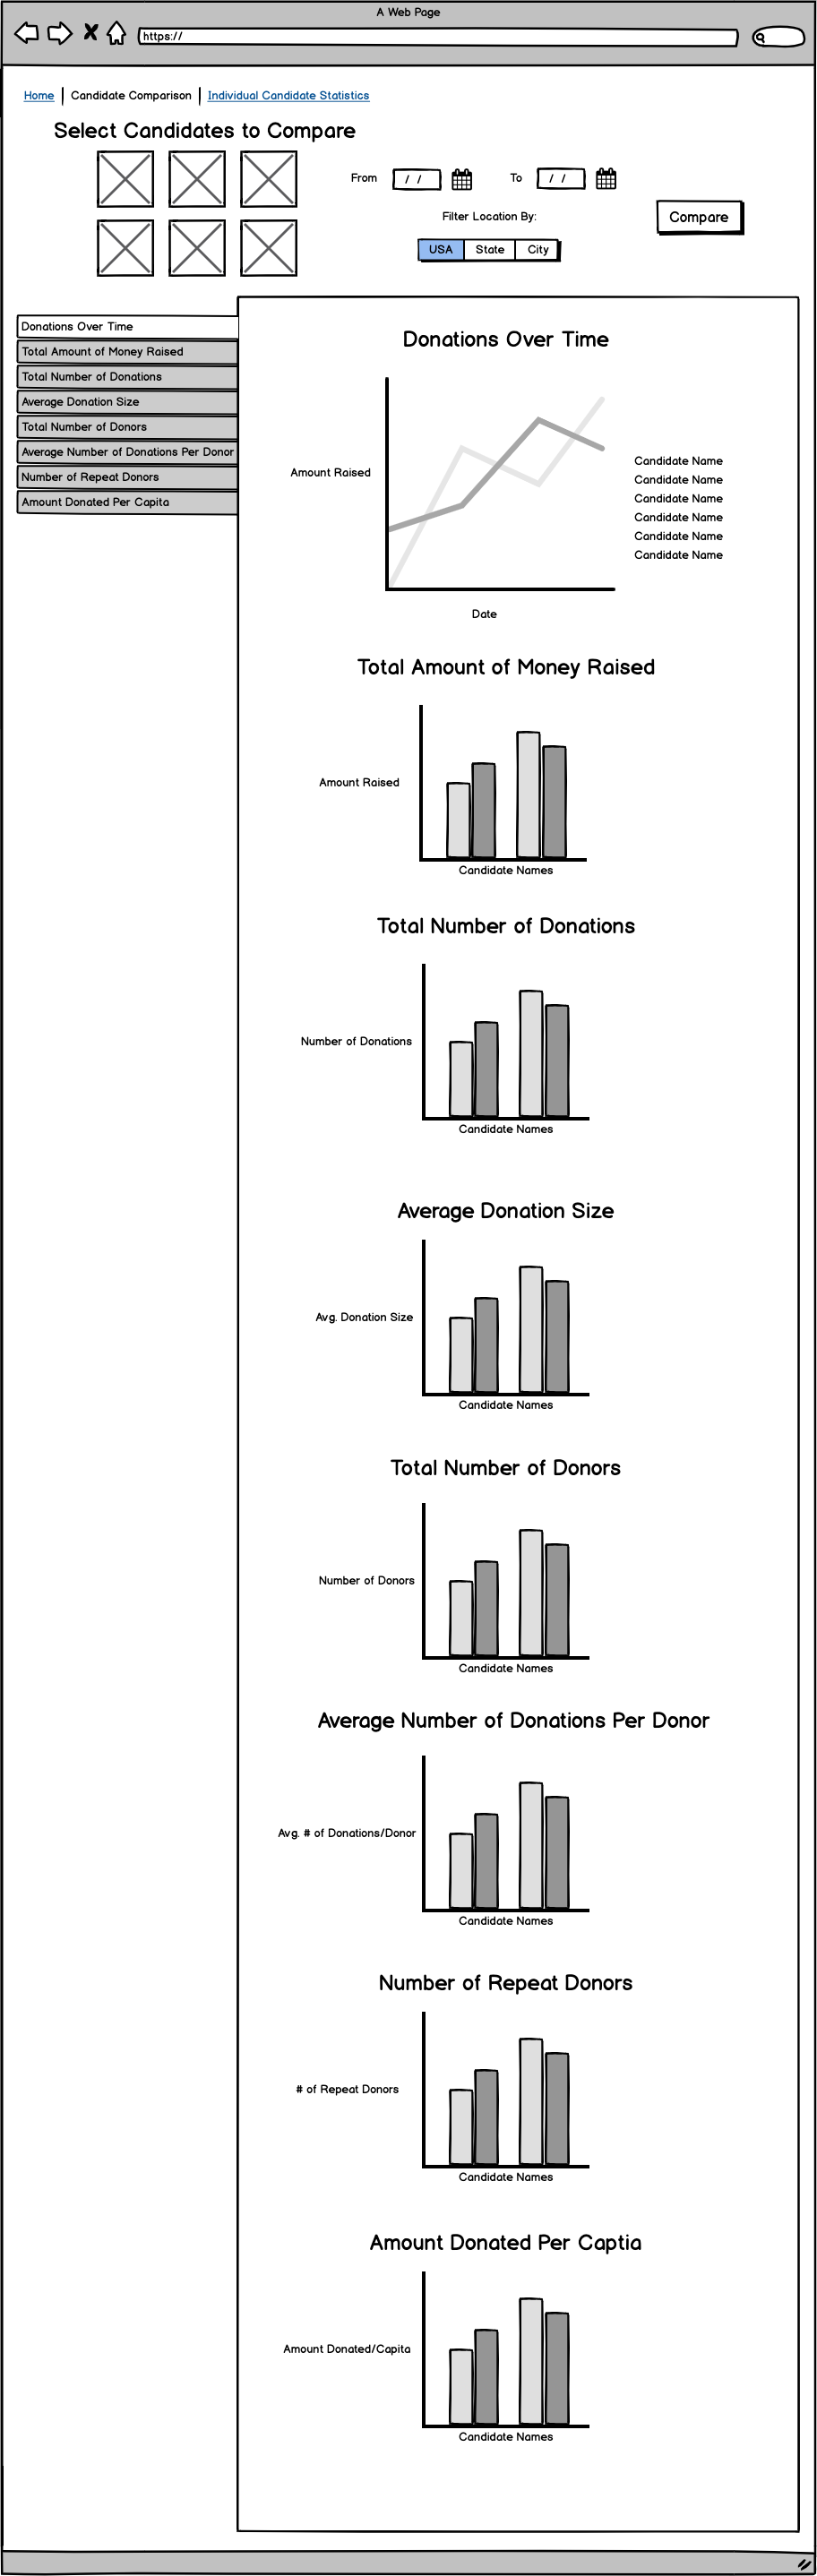
\includegraphics[scale=.20]{candidatecompbyus}
        \caption{Candidate comparison, whole country.}
        \label{fig:2}
        \end{center}
    \end{figure}
    \begin{figure}[H]
        \begin{center}
        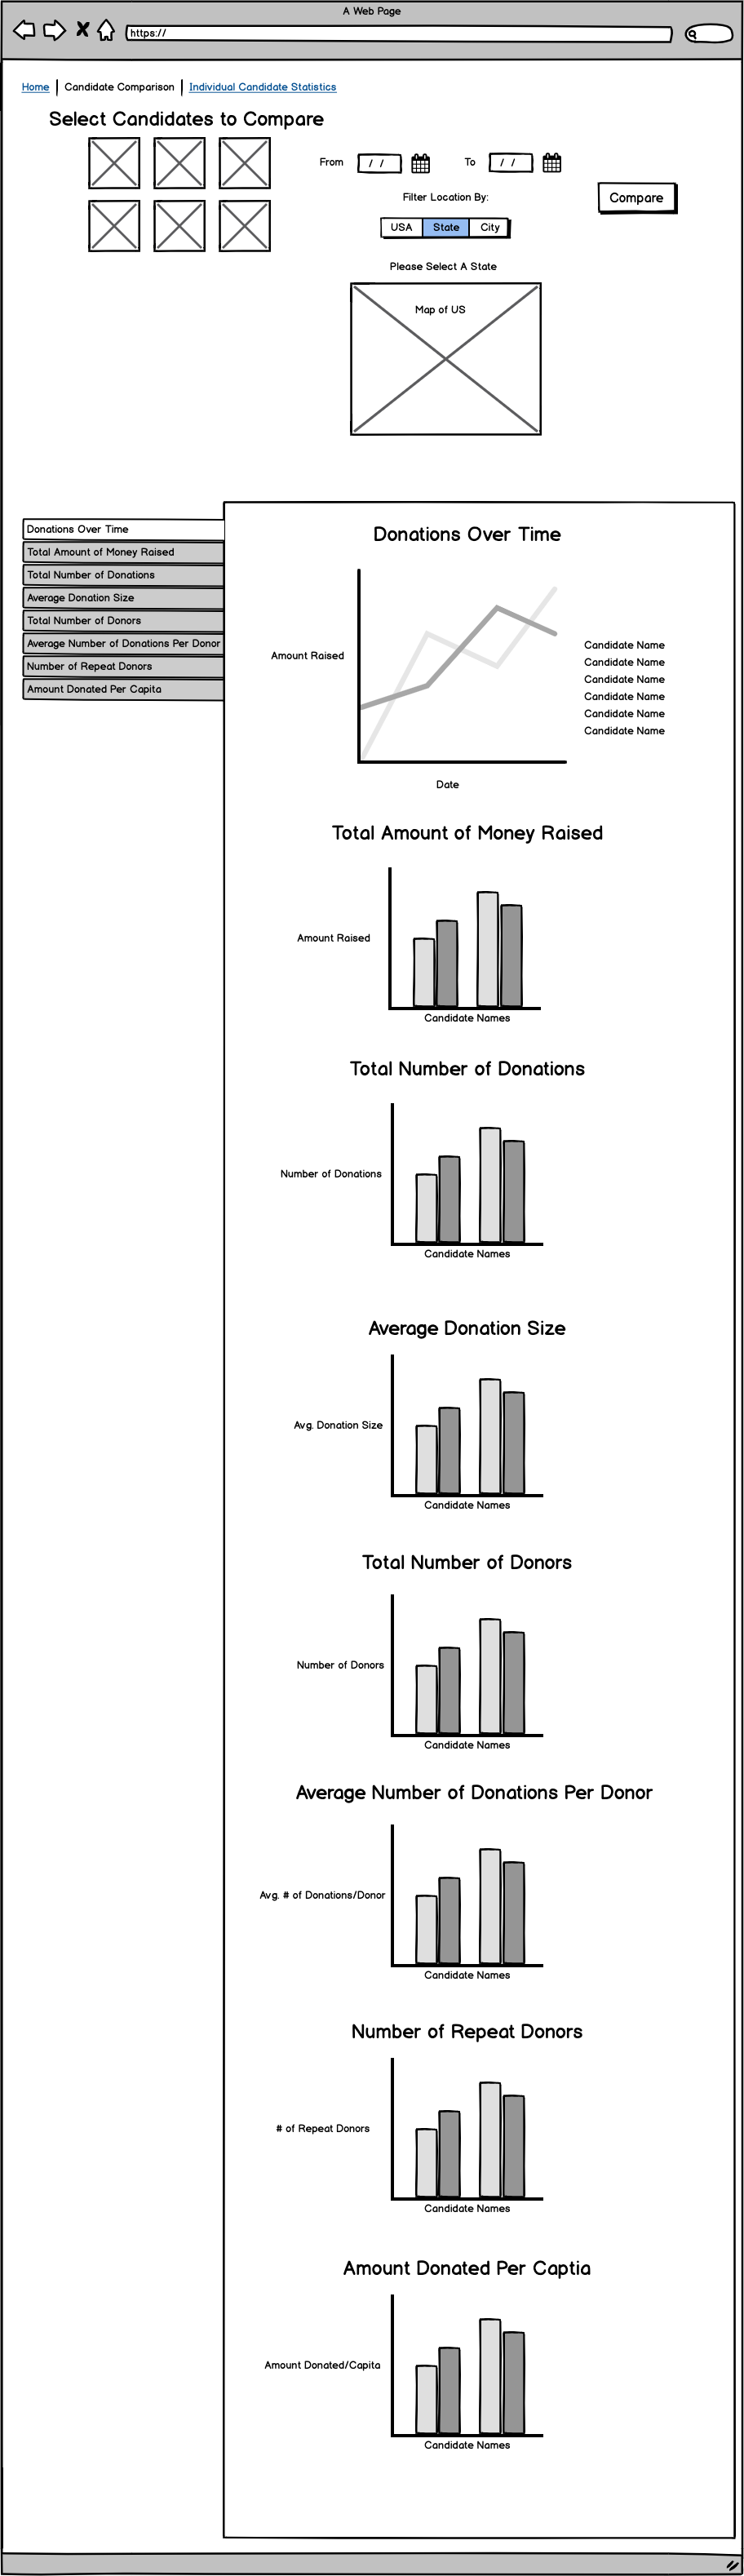
\includegraphics[scale=.20]{candidatecompbystate}
        \caption{Candidate comparison, by state.}
        \label{fig:3}
        \end{center}
    \end{figure}
    \begin{figure}[H]
        \begin{center}
        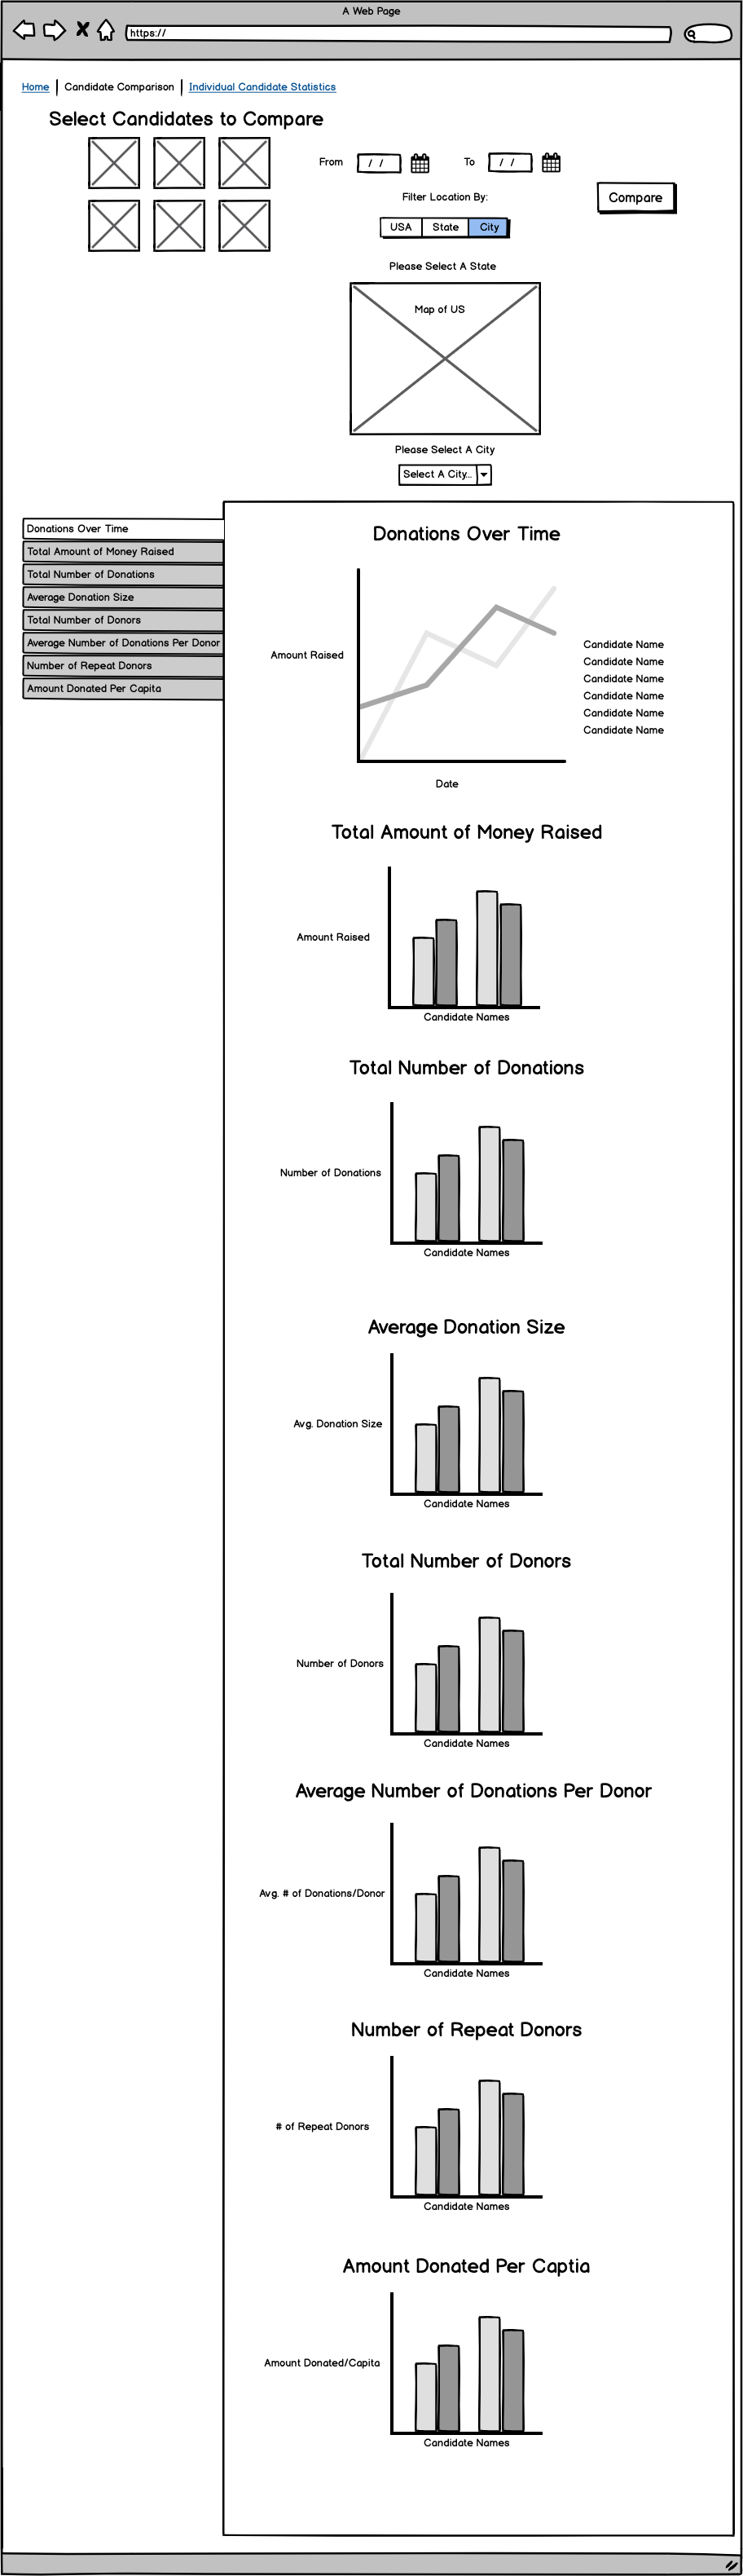
\includegraphics[scale=.20]{candidatecompbycity}
        \caption{Candidate comparison, by city.}
        \label{fig:4}
        \end{center}
    \end{figure}
    If the user selects the ``Candidate Comparison’’ link, they will be directed to that page (Figure \ref{fig:2}). From there the user has the option of what candidates the user would like to compare. The user can choose to compare as few as two candidates or up to all candidates at once. The user will then select the date range and location that they would like the data to be analysed. Figure \ref{fig:2} shows what it would look like if ``US’’ was selected. If ``State’’ (Figure \ref{fig:3} or ‘’City`` (Figure \ref{fig:4} are selected then a map of the US will appear and the user can select the specific state. If ``City’’ was selected, then once a state is selected, a searchable drop down of all available cities in that state will appear. Once the location is specified, the user would then select ``Compare’’. As shown in Figures \ref{fig:2}-\ref{fig:4}, the following graphs would be generated: Donations Over Time, Total Amount of Money Raised, Total Number of Donations, Average Donation Size, Total Number of Donors, Average Number of Donations Per Donor, Number of Repeat Donors, and Amount Donated Per Capita (depending on if you selected ``USA’’, ``State’’, or ``City’’).

    \subsection{Candidate Statistics}
    \begin{figure}[H]
        \begin{center}
        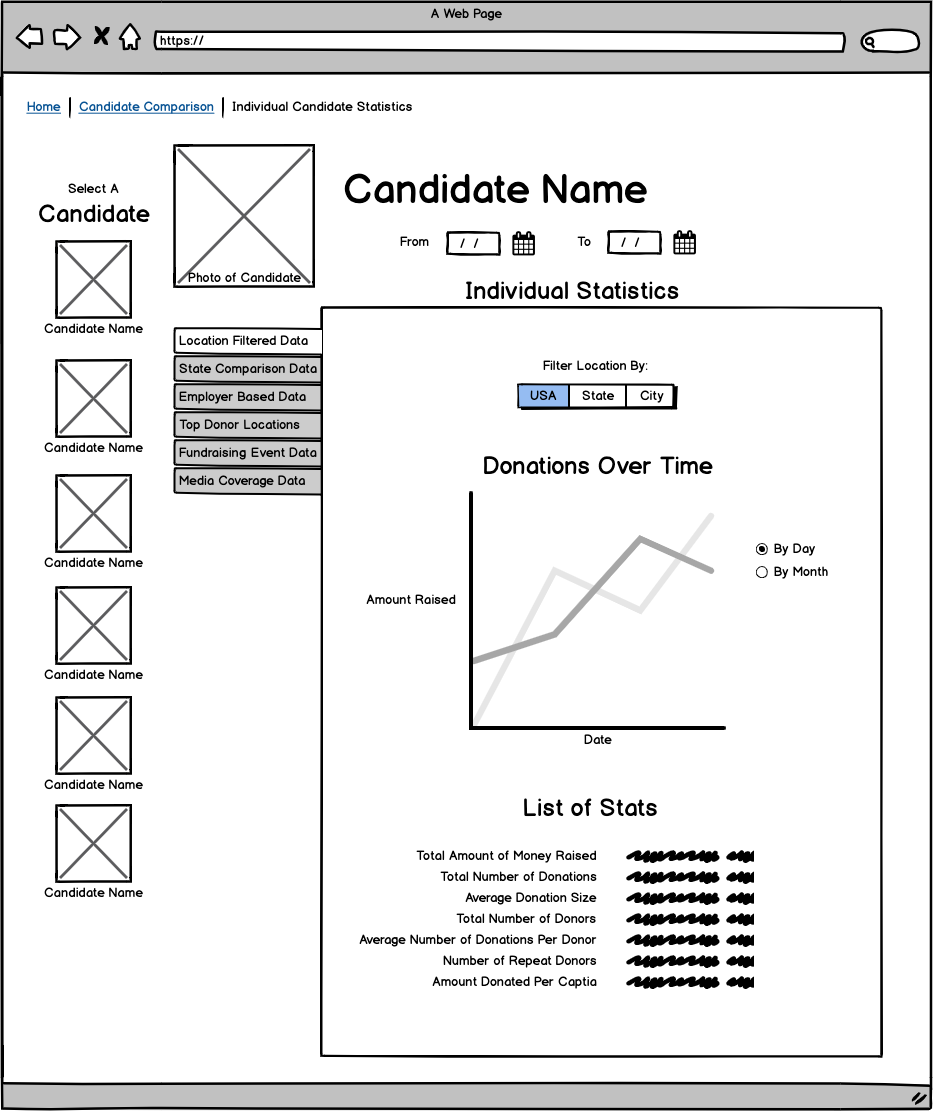
\includegraphics[scale=.30]{candidatefilterusday}
        \caption{Individual candidate, whole country by date.}
        \label{fig:5}
        \end{center}
    \end{figure}
    
    \begin{figure}[H]
        \begin{center}
        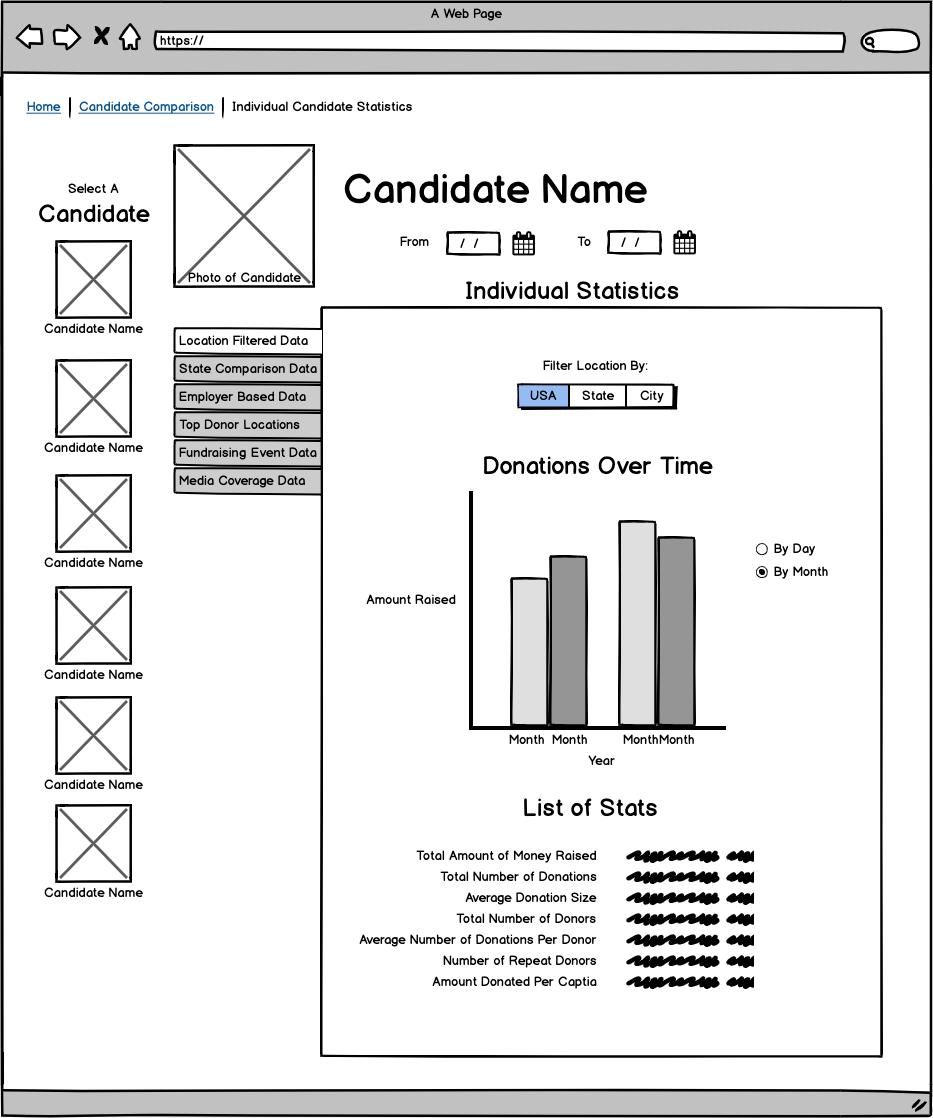
\includegraphics[scale=.30]{candidatefilterusmonth}
        \caption{Individual candidate, whole country by month.}
        \label{fig:6}
        \end{center}
    \end{figure}
    
    \begin{figure}[H]
        \begin{center}
        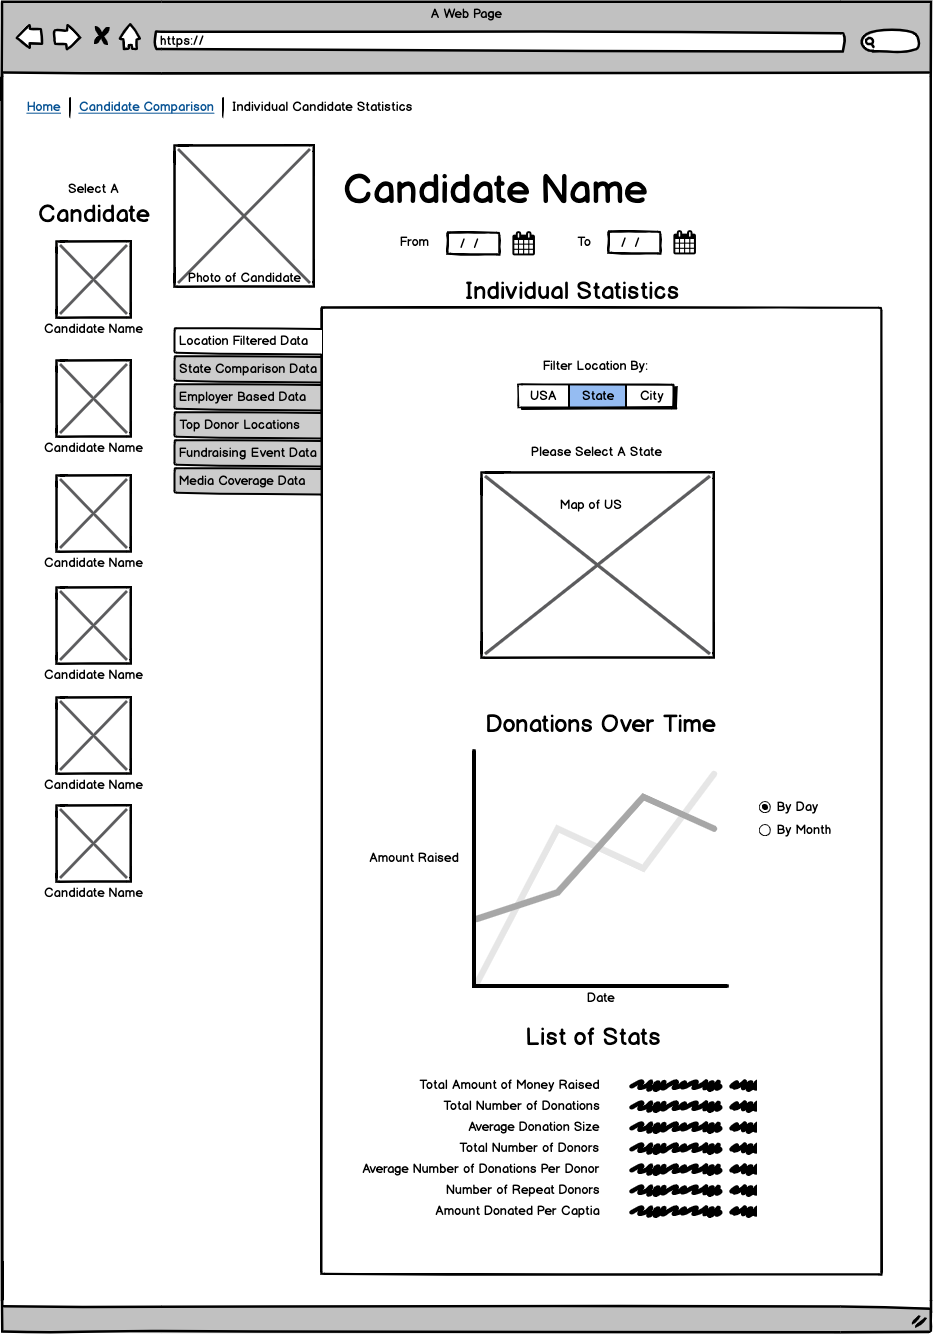
\includegraphics[scale=.30]{candidatefilterstateday}
        \caption{Individual candidate, by state and date.}
        \label{fig:7}
        \end{center}
    \end{figure}
    
    \begin{figure}[H]
        \begin{center}
        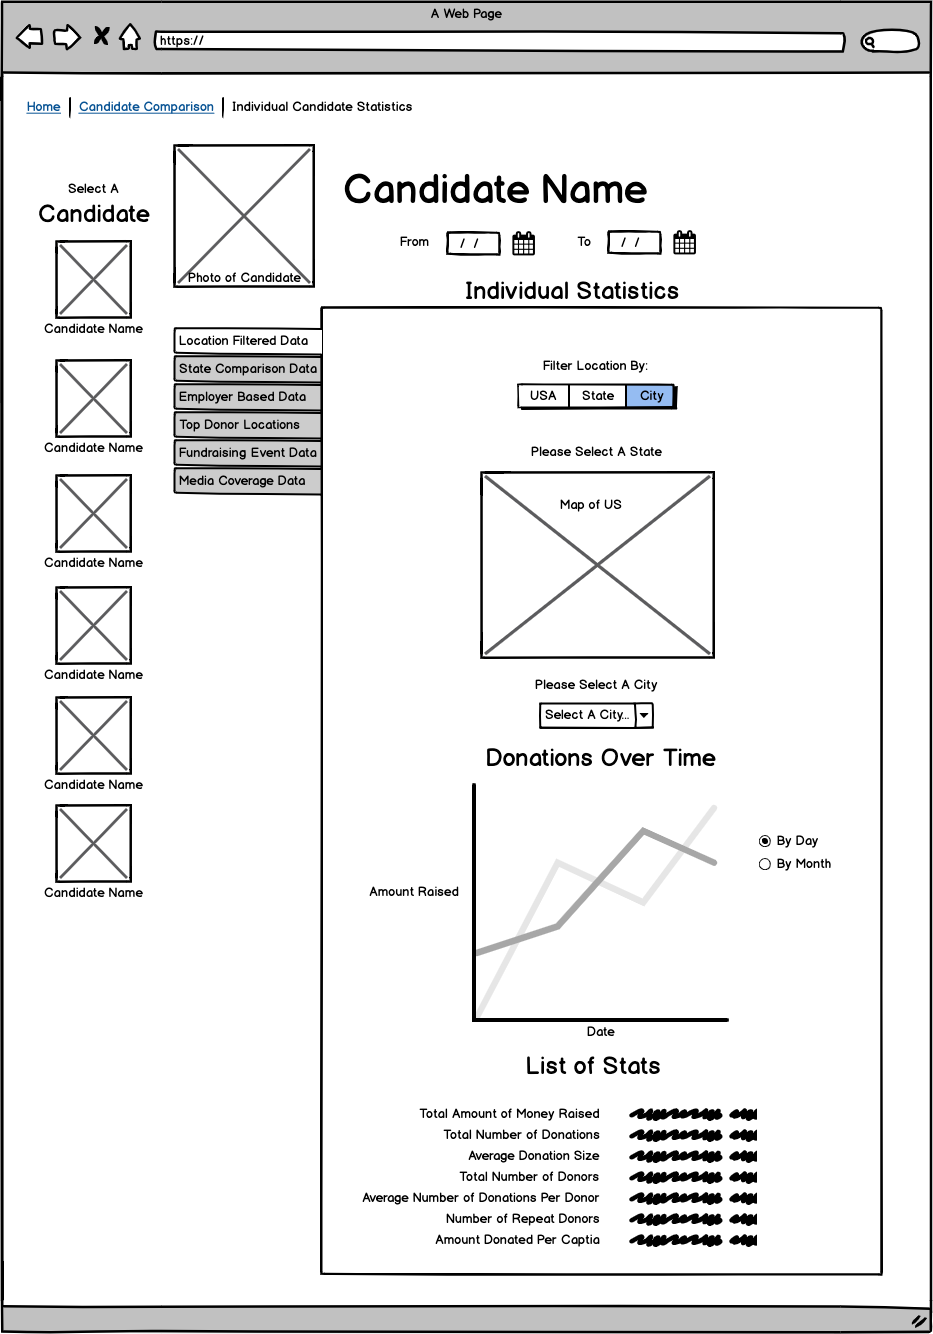
\includegraphics[scale=.3]{candidatefiltercityday}
        \caption{Individual candidate by city and date.}
        \label{fig:8}
        \end{center}
    \end{figure}
    
  The user can also look at individual statistics for a candidate by navigating to the ``Individual Candidate Statistics’’ page. When the page is initially loaded, the default dates will be selected (earliest donation to most recent donation) and the default tab will be loaded (``Location Filtered Data’’), with location set to ``USA’’, and the statistics will be generated based on that date range and location (Figure \ref{fig:5}). This “Location Filtered Data” is the same data that is generated in the “Candidate Comparison” page but for just one candidate instead of many. Figure \ref{fig:6} shows an option that will be available for the Donation Over Time graph that will allow the user to select between a line graph that shows daily donation totals vs. a bar graph that will show monthly donation totals. Once again, Figures \ref{fig:7} and \ref{fig:8} show the different location selection options similar to the ``Candidate Comparison’’ page.

    \begin{figure}[H]
        \begin{center}
        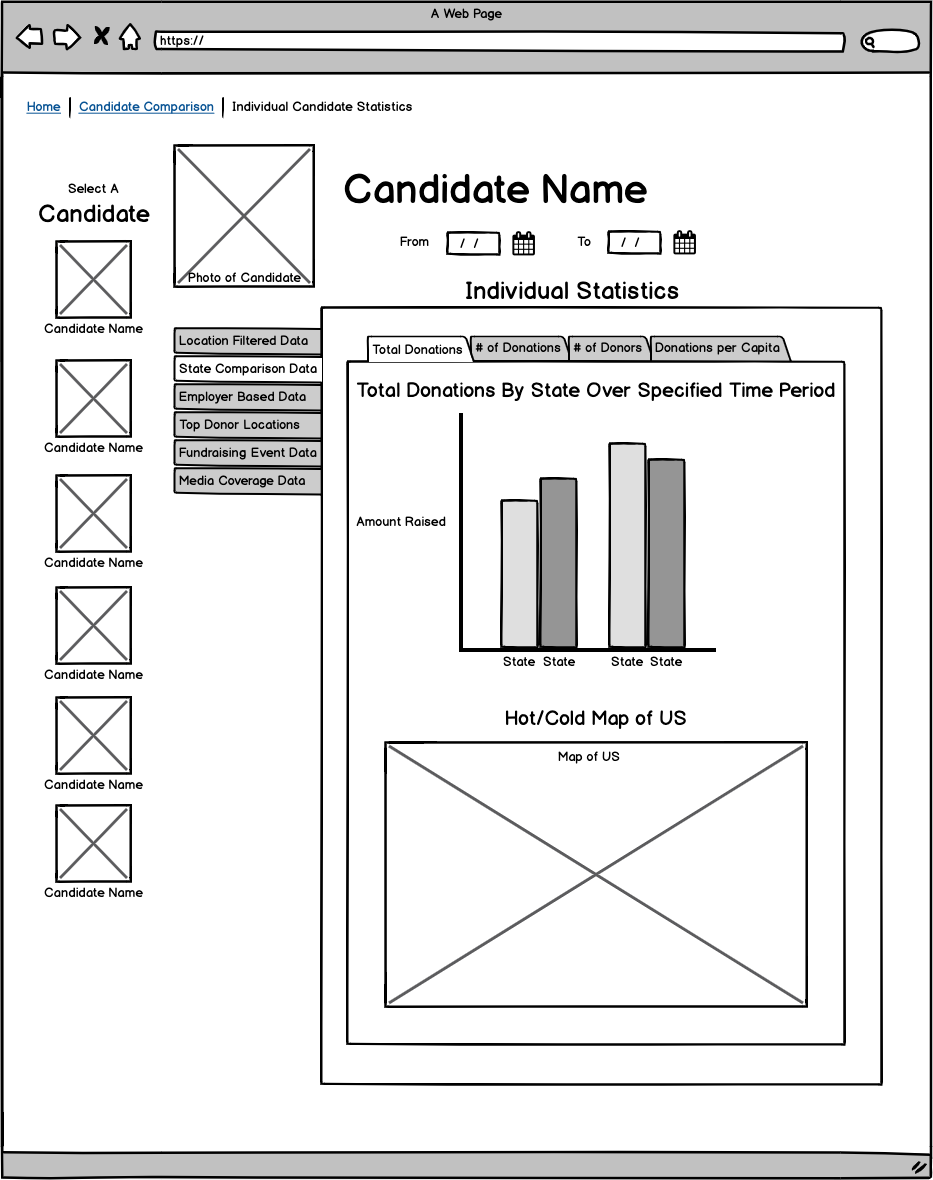
\includegraphics[scale=.30]{candidatestate}
        \caption{Individual candidate, state comparison data.}
        \label{fig:9}
        \end{center}
    \end{figure}
    The user will then be able to select the ``State Comparison Data’’ tab to look at a number of data comparisons by state (Figure \ref{fig:9}). Each of these four comparisons (Total Donations, \# of Donations, \# of Donors, and Donations Per Capita) will display a bar graph showing all 50 states in descending order and a US ``heat map’’ showing different colors for different states based on the item being compared.
    \begin{figure}[H]
        \begin{center}
        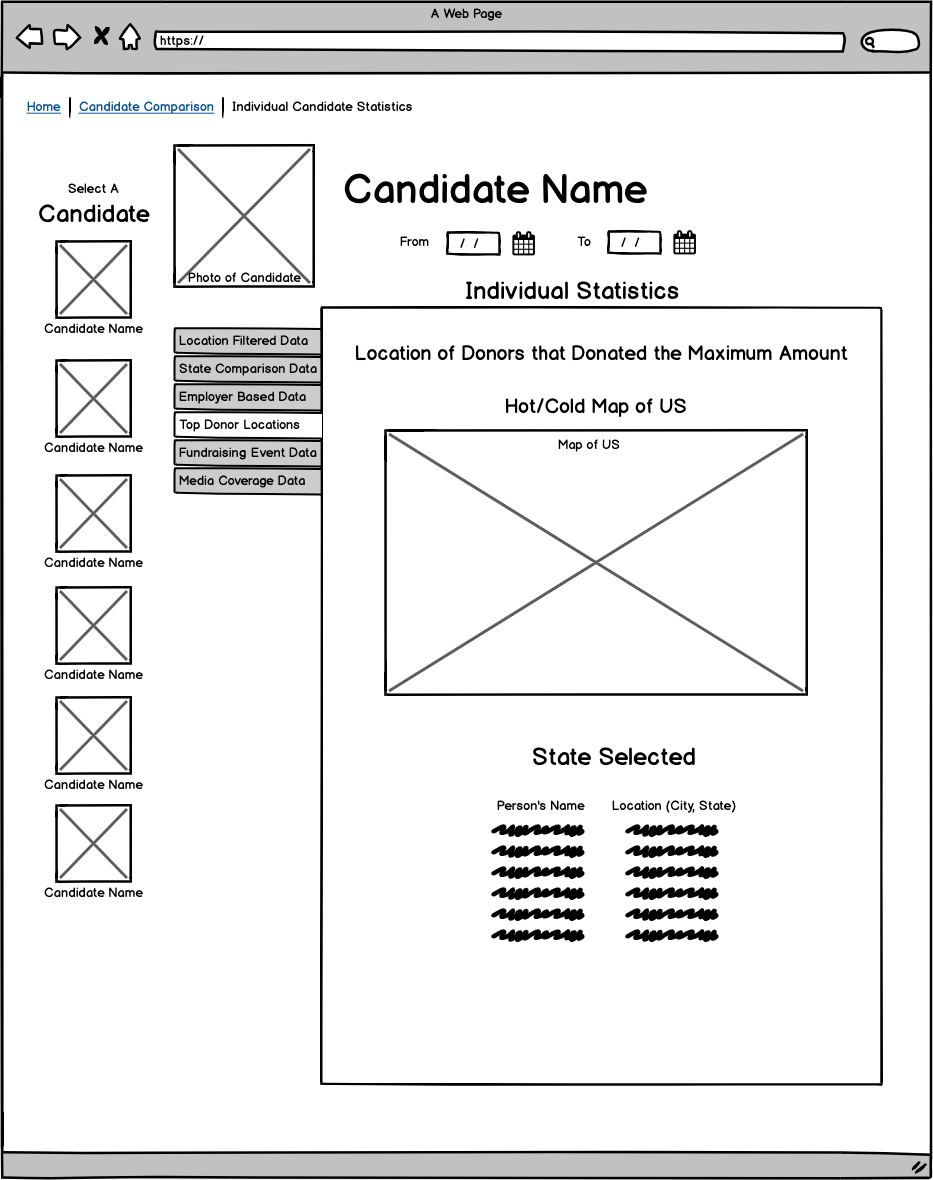
\includegraphics[scale=.30]{candidatetopdonor}
        \caption{Individual candidate, top donors.}
        \label{fig:10}
        \end{center}
    \end{figure}
    The ``Top Donor Locations’’ tab will have another US ``heat map’’ showing the locations of donors that contributed the maximum amount to the campaign, which is \$2,800/individual for a Presidential Primary campaign (Figure \ref{fig:10}). If the user selects a specific state, a list of the individuals that donated the maximum amount in that state will appear below the map.

    \begin{figure}[H]
        \begin{center}
        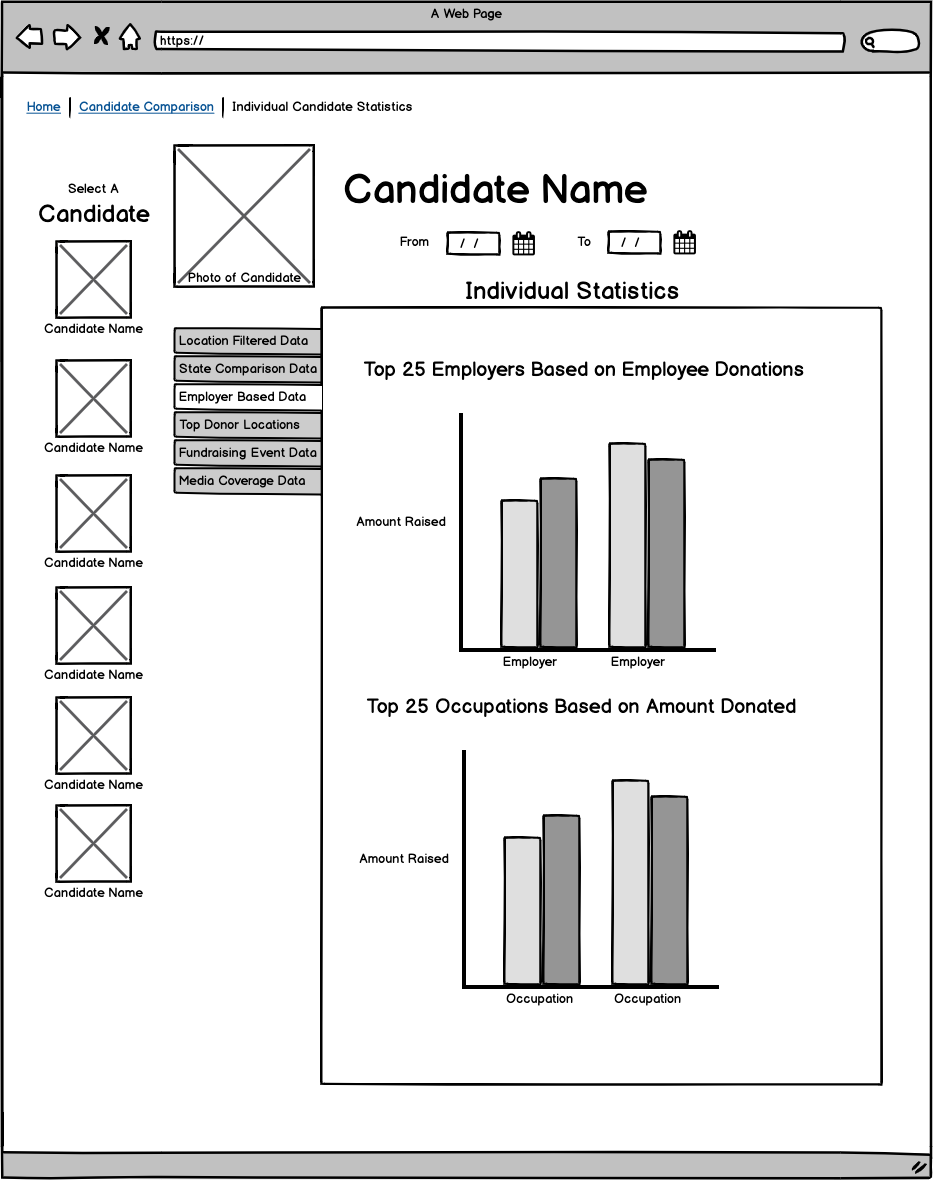
\includegraphics[scale=.30]{candidateemployer}
        \caption{Individual candidate by employer.}
        \label{fig:11}
        \end{center}
    \end{figure}
    The next tab,``Employer Based Data’’, will have two bar graphs showing the top 25 employers based on employee donations and top 25 occupations based on amount donated (Figure \ref{fig:11})
    \begin{figure}[H]
        \begin{center}
        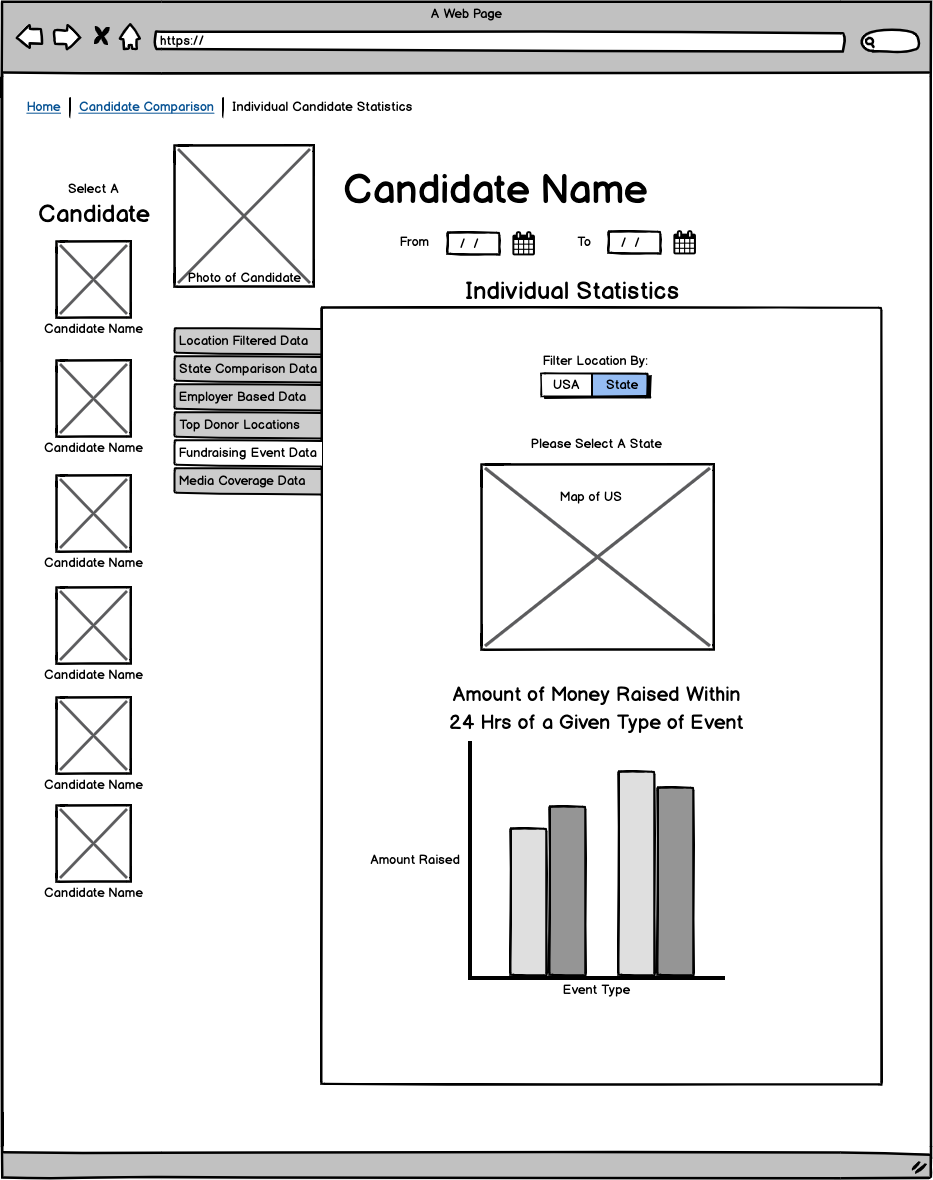
\includegraphics[scale=.30]{candidateevent}
        \caption{Individual candidate, event comparison.}
        \label{fig:12}
        \end{center}
    \end{figure}
    The ``Fundraising Event Data’’ tab will focus on comparing the amount of money donated within 24 hrs of a given type of fundraising event (i.e. public speech, town hall meeting, dinner, etc.). The user will be able to filter the event data by the entire US or by state.

    \begin{figure}[H]
        \begin{center}
        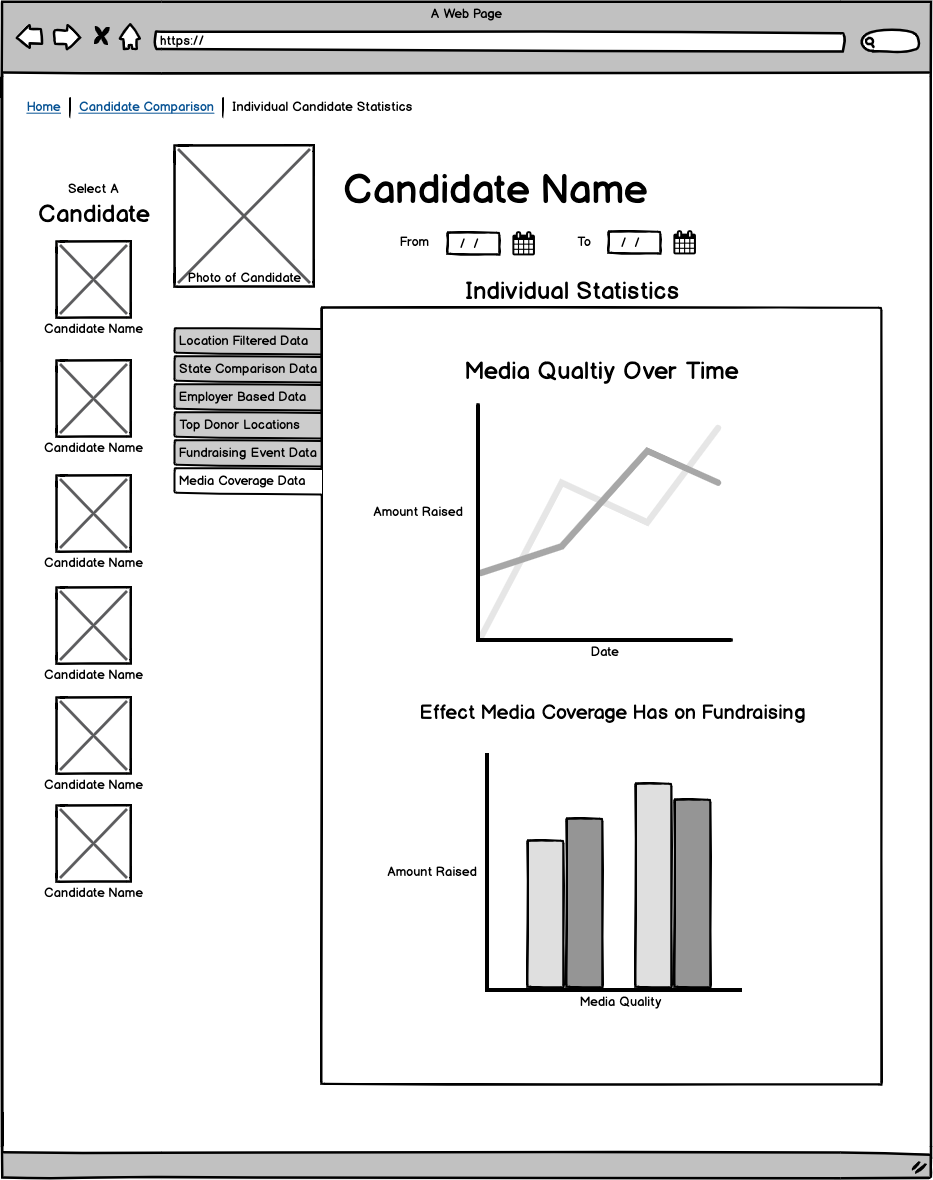
\includegraphics[scale=.30]{candidatemedia}
        \caption{Individual candidate, media coverage data.}
        \label{fig:13}
        \end{center}
    \end{figure}
    The ``Media Coverage Data’’ tab will focus on the quality of news coverage the candidate receives on a given day. If the coverage is positive, it will be labeled as +1, neutral labeled 0, and negative labeled -1. This coverage quality will be displayed cumulatively as a line graph over the specified date range. Also a bar graph will display the the total amount of money donated within 24 hrs of a given type of coverage (positive, neutral, or negative).
\section{ER Diagram}
    \begin{figure}[H]
        \begin{center}
        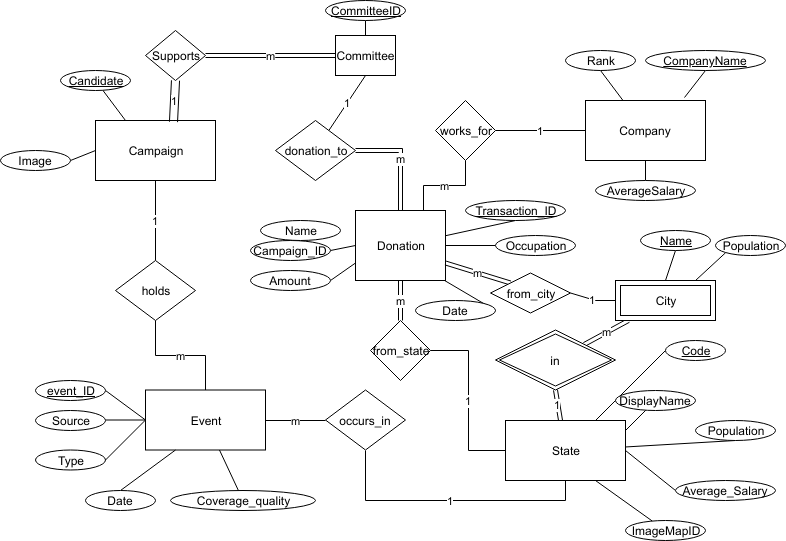
\includegraphics[scale=.40]{projecter}
        \caption{Project's ER diagram}
        \label{fig:ER Diagram}
        \end{center}
    \end{figure}

    \subsection{Donation}
    While the FEC does provide substantial information about the donors to a campaign, there is insufficient data to uniquely identify an individual. A sample of the data provided by the FEC is included in figure \ref{fig:fecdata}. With such a large data set as all political donors, the combination of name, zip-code, employer, and occupation seem to be insufficiently unique to provide a primary key specific to an individual. Furthermore, inconsistencies in how this information may be submitted by an individual makes this task near impossible. This limitation in our data will have to be accounted for in the queries that we provide. 
        \begin{figure}[H]
            \begin{center}
            \includegraphics[scale=.30]{FECdata}
            \caption{Sample FEC data}
            \label{fig:fecdata}
            \end{center}
        \end{figure}
    \subsection{Campaign and Committee}
    Each presidential candidate has a principal campaign committee. The organization most directly under the control of a candidate. Often times, donations are sent to smaller committees that are established by a campaign to manage efforts in a geographic area or demographic. Each committee that we can find that supports a specific candidate, should be added to the Committee table, using the candidate's name as a foreign key. We will use integrity constraints to ensure that the candidate matches an available candidate. Our use model for the application does not concern itself with which specific committee was donated to, but rather the general level of support a candidate has measured through donations. Therefore, the distinction between a candidate and the committees that support them will be abstracted away from our users. 
    \subsection{Company}
    While we cannot expect to obtain information related to every possible response to the prompt for an employer, we expect to find relevant information for some large employers. It is also important to consider that when provided by the donor, the employer specified is a text entry. We expect significant variations between company names intended to reference the same entity, e.g. ``Employer Inc.'' and ``Employer'' appearing in the donation data. It may be necessary to utilize an additional table mapping multiple company aliases to a single tuple in the company table. 
    \subsection{Events}
    One of the primary motivators for queries in our application is the effect of events and news stories on campaign donations. To track these we will need to import a list of events. Ballotpedia provides a list of such events for each candidate, along with the date. We intend to leverage the information provided by Ballotpedia into a functional table. A sample of the data from Ballotpedia is available in figure \ref{fig:events}. Additional data about the type of event and whether media coverage was ``good'' or``bad'' will be stored. 
        \begin{figure}[H]
            \begin{center}
            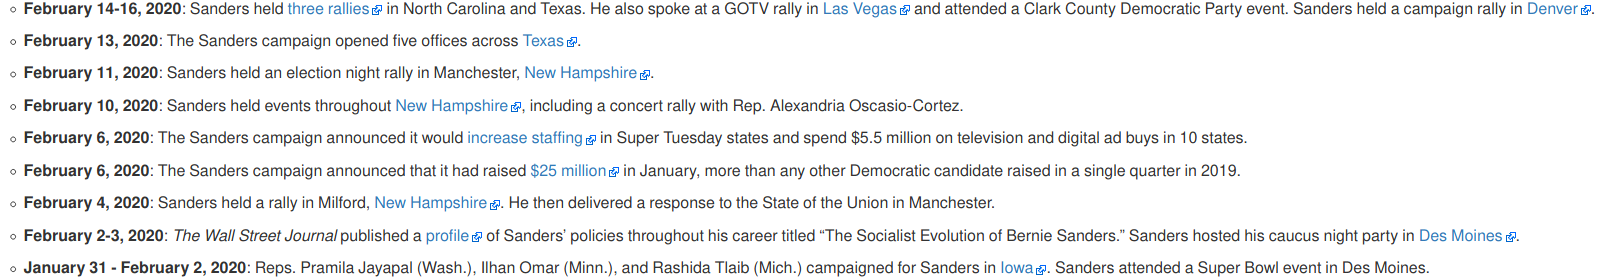
\includegraphics[scale=.40]{events}
            \caption{Sample event list}
            \label{fig:events}
            \end{center}
        \end{figure}
    \subsection{Location}
    Since our key idea relates the effect of events and news stories on donations, we feel it is a key aspect to track how an event or news story specific to a state effects the contributions from donors in that state. This will enable us to engage in queries such as ``Does an event in a state with a higher per capita income lead to more donations than an event in a state with less per capita income?'' While donations are trackable to specific city, the effect of events are often not limited to a single locality. For this reason, we are not pinpointing an event to a specific city, but instead merely the state in which the event took place. 
\end{document}

